\documentclass{article}
\usepackage{graphicx, amsmath, amssymb, mathtools, fancyhdr,float} % Required for inserting images

\graphicspath{{Images/}}

\setlength{\oddsidemargin}{0in}
\setlength{\textwidth}{6.5in}
\setlength{\topmargin}{-.55in}
\setlength{\textheight}{9in}
\pagestyle{fancy}

\fancyfoot{}
\fancyhead[R]{\thepage}
\fancyhead[L]{Nonlinear Waves RG}


\begin{document}

\begin{center}
    {\Huge Nonlinear Waves HW 1}
    \vspace{0.5cm}

    {\Large Michael Nameika}
\end{center}


\begin{itemize}
    \item[1.] Recreate Figure 1.6.
    \newline\newline
    \begin{center}
        \begin{figure}[H]
            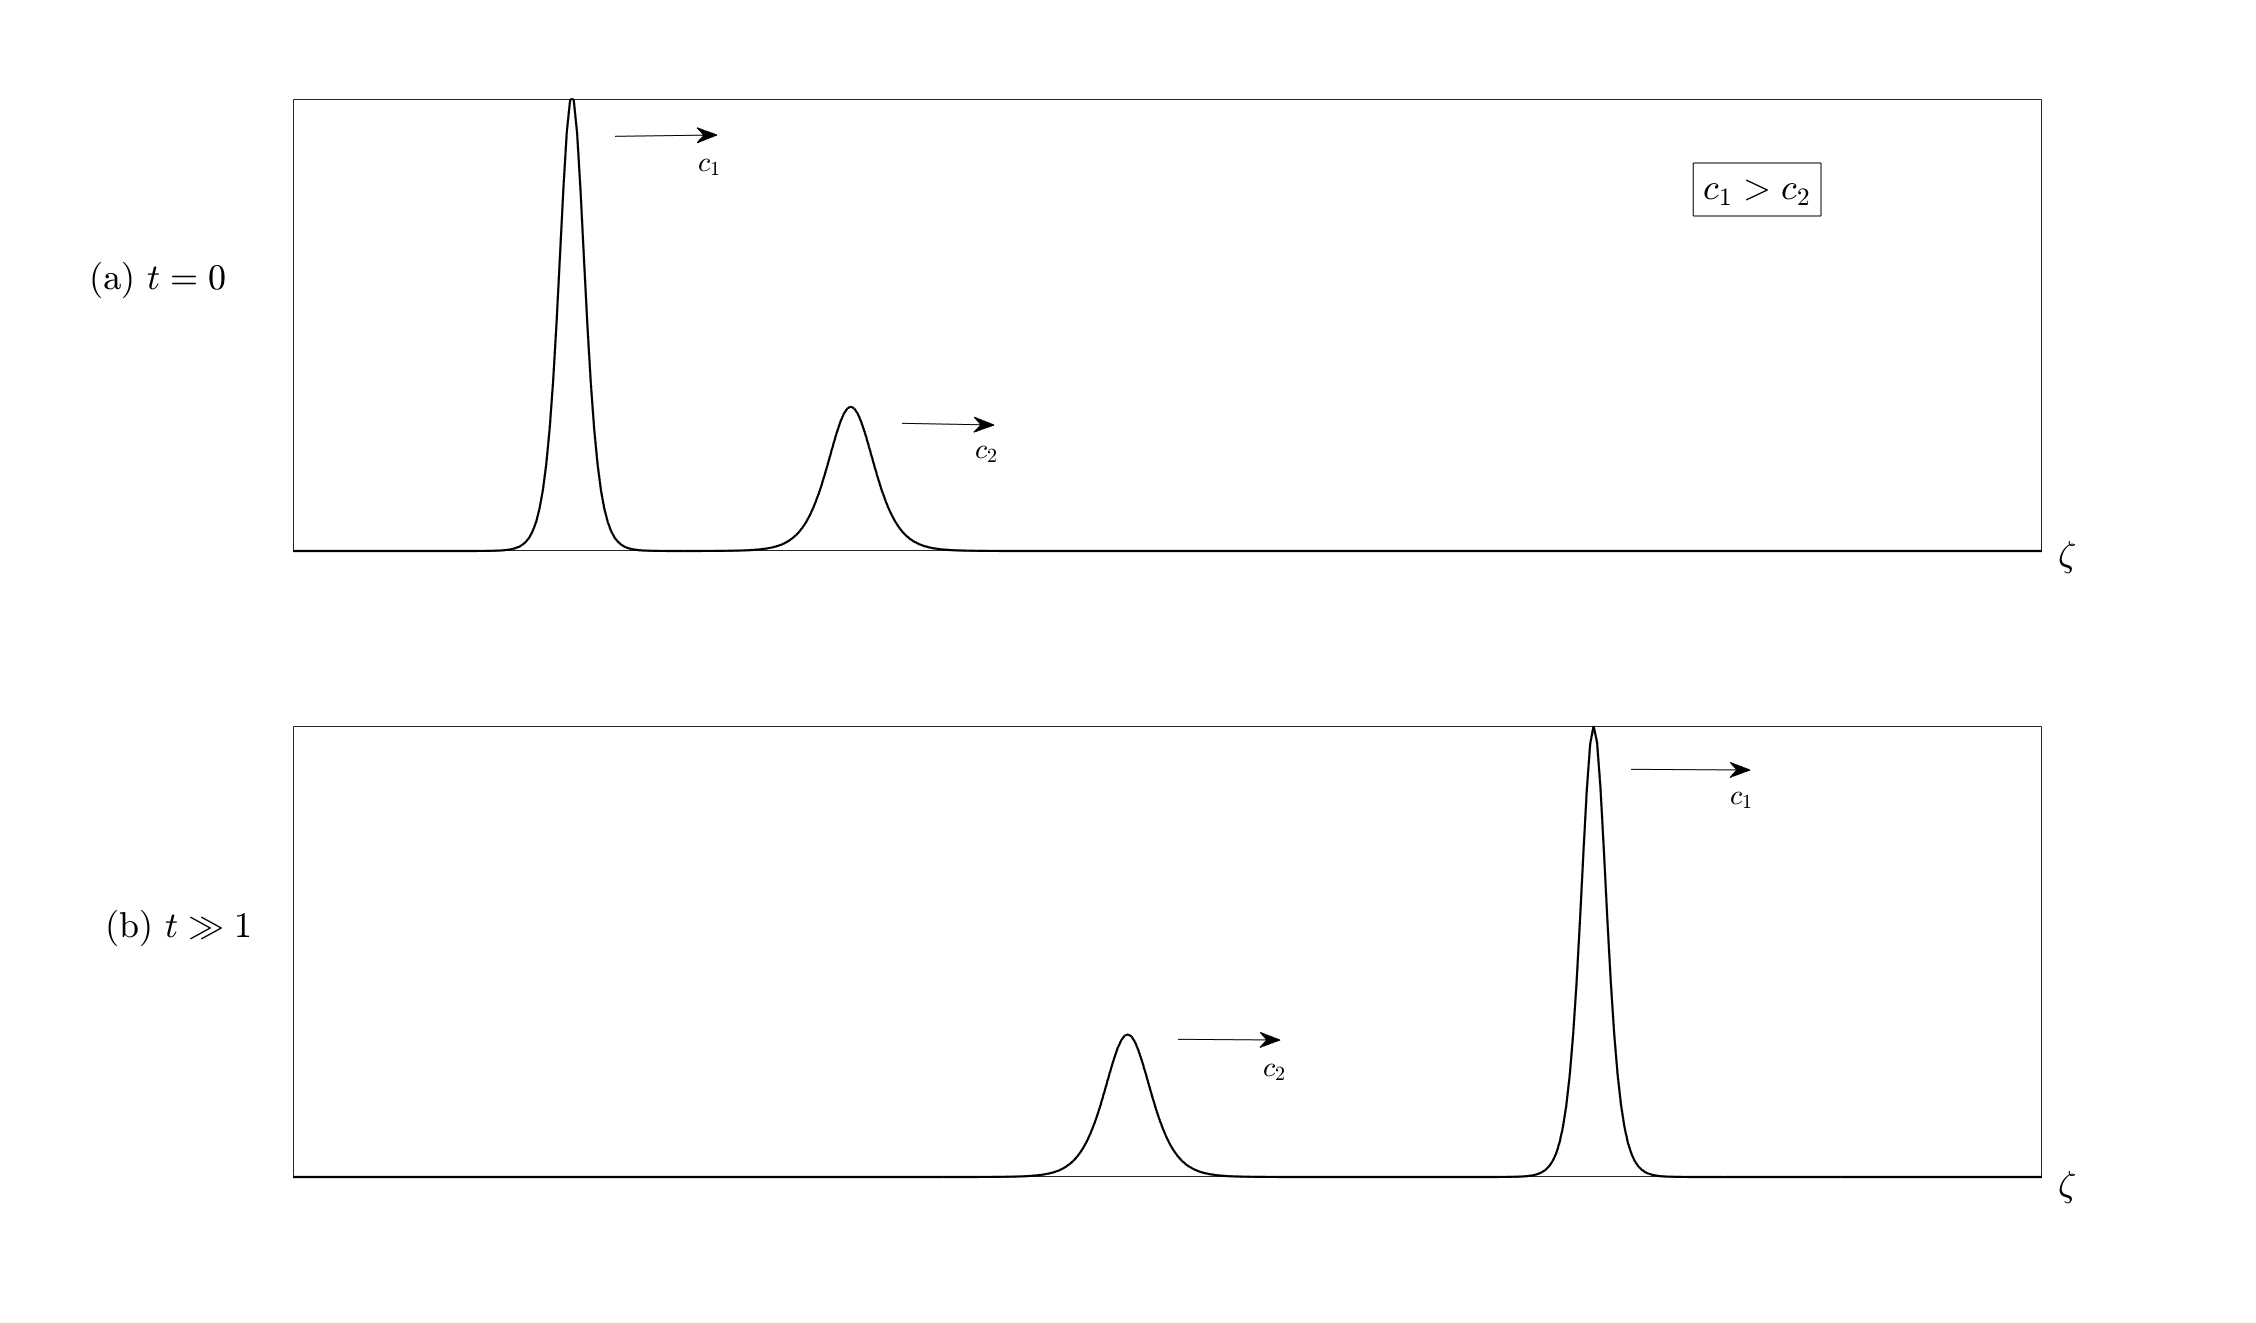
\includegraphics[scale = 0.25]{elastic_solitons.png}
            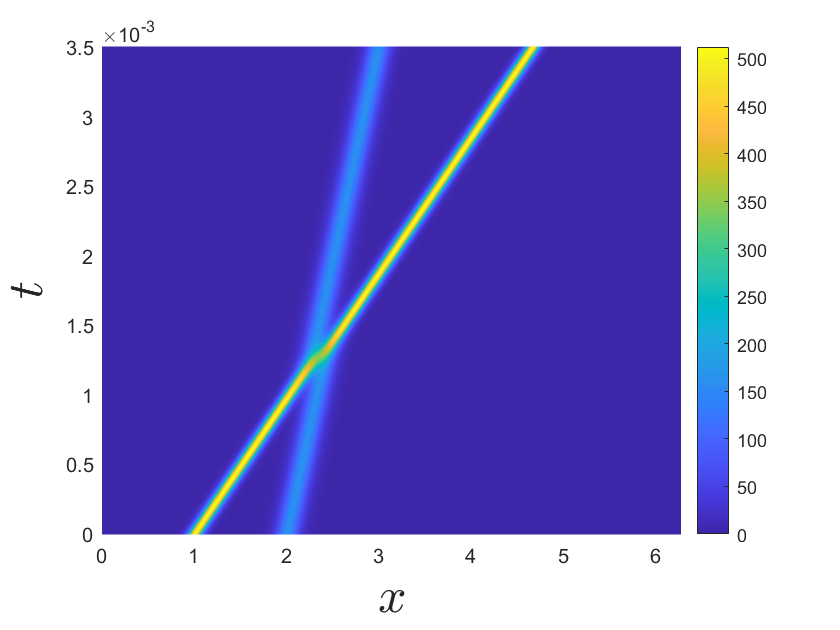
\includegraphics[scale = 0.5]{soliton_interaction_waterfall.png}
            \caption{Above: elastic soliton interaction. Below: waterfall plot of soliton interactions}
        \end{figure}
    \end{center}

    \item[2.] Given the modificed KdV (mKdV) equation
    \[u_t + 6u^2u_x + u_{xxx} = 0,\]
    reduce the problem to an ODE by investigating traveling wave solutions of the form: $u = U(x-ct)$.
    \newline\newline
    \textit{Soln.} Suppose $u = U(x-ct)$ and let $\zeta = x - ct$. Then
    \begin{align*}
        \frac{\partial u}{\partial t} &= \frac{dU}{d\zeta}\frac{\partial \zeta }{\partial t} = -c\frac{dU}{d\zeta}\\
        \frac{\partial u}{\partial x} &= \frac{dU}{d\zeta}\frac{\partial \zeta}{\partial x} = \frac{dU}{d\zeta}\\
        \implies \frac{\partial^3u}{\partial x^3} &= \frac{d^3U}{d\zeta^3}.
    \end{align*}
    Thus the mKdV equation becomes
    \[-c\frac{dU}{d\zeta} + 6U^2\frac{dU}{d\zeta} + \frac{d^3U}{d\zeta^3} = 0.\]
    Notice that $6u^2\frac{dU}{d\zeta} = 2\frac{d}{d\zeta}\left(U^3\right)$ so the above equation becomes
    \[-c\frac{dU}{d\zeta} + 2\frac{d}{d\zeta}\left(U^3\right) + \frac{d^3U}{d\zeta} = 0.\]
    Integrating once yields
    \[-cU + 2U^3 + \frac{d^2U}{d\zeta} = E_1\]
    where $E_1$ is a constant of integration. Multiply each side by $\frac{dU}{d\zeta}$ and integrate again to get
    \begin{align*}
        -\frac{c}{2}U^2 + \frac{1}{2}U^4 + \frac{1}{2}\left(\frac{\partial U}{\partial \zeta}\right)^2 &= E_1u + E_2\\
        -cU^2 + U^4 + \left(\frac{\partial u}{\partial \zeta}\right)^2 &= \tilde{E}_1U + \tilde{E}_2
    \end{align*}
    where $\tilde{E}_{1,2} = 2E_{1,2}$. Isolating $\frac{dU}{d\zeta}$ gives 
    \begin{align*}
        \left(\frac{\partial U}{\partial \zeta}\right)^2 &= -U^4 + cU^2 + \tilde{E}_1U + \tilde{E}_2\\
        &= P_4(U)
    \end{align*}
    where $P_4(U) = -U^4 + cU^2 + \tilde{E}_1U + \tilde{E}_2$.
    \begin{itemize}
        \item[(a)] Express the bounded periodic solutions in terms of Jacobi elliptic functions.
        \newline\newline
        \textit{Soln.} We now assume that $P_4$ splits, that is, there exist roots $\alpha \leq \beta \leq \gamma \leq \delta$ such that
        \[P_4(U) = -(U-\alpha)(U-\beta)(U-\gamma)(U - \delta).\]
        \begin{center}
            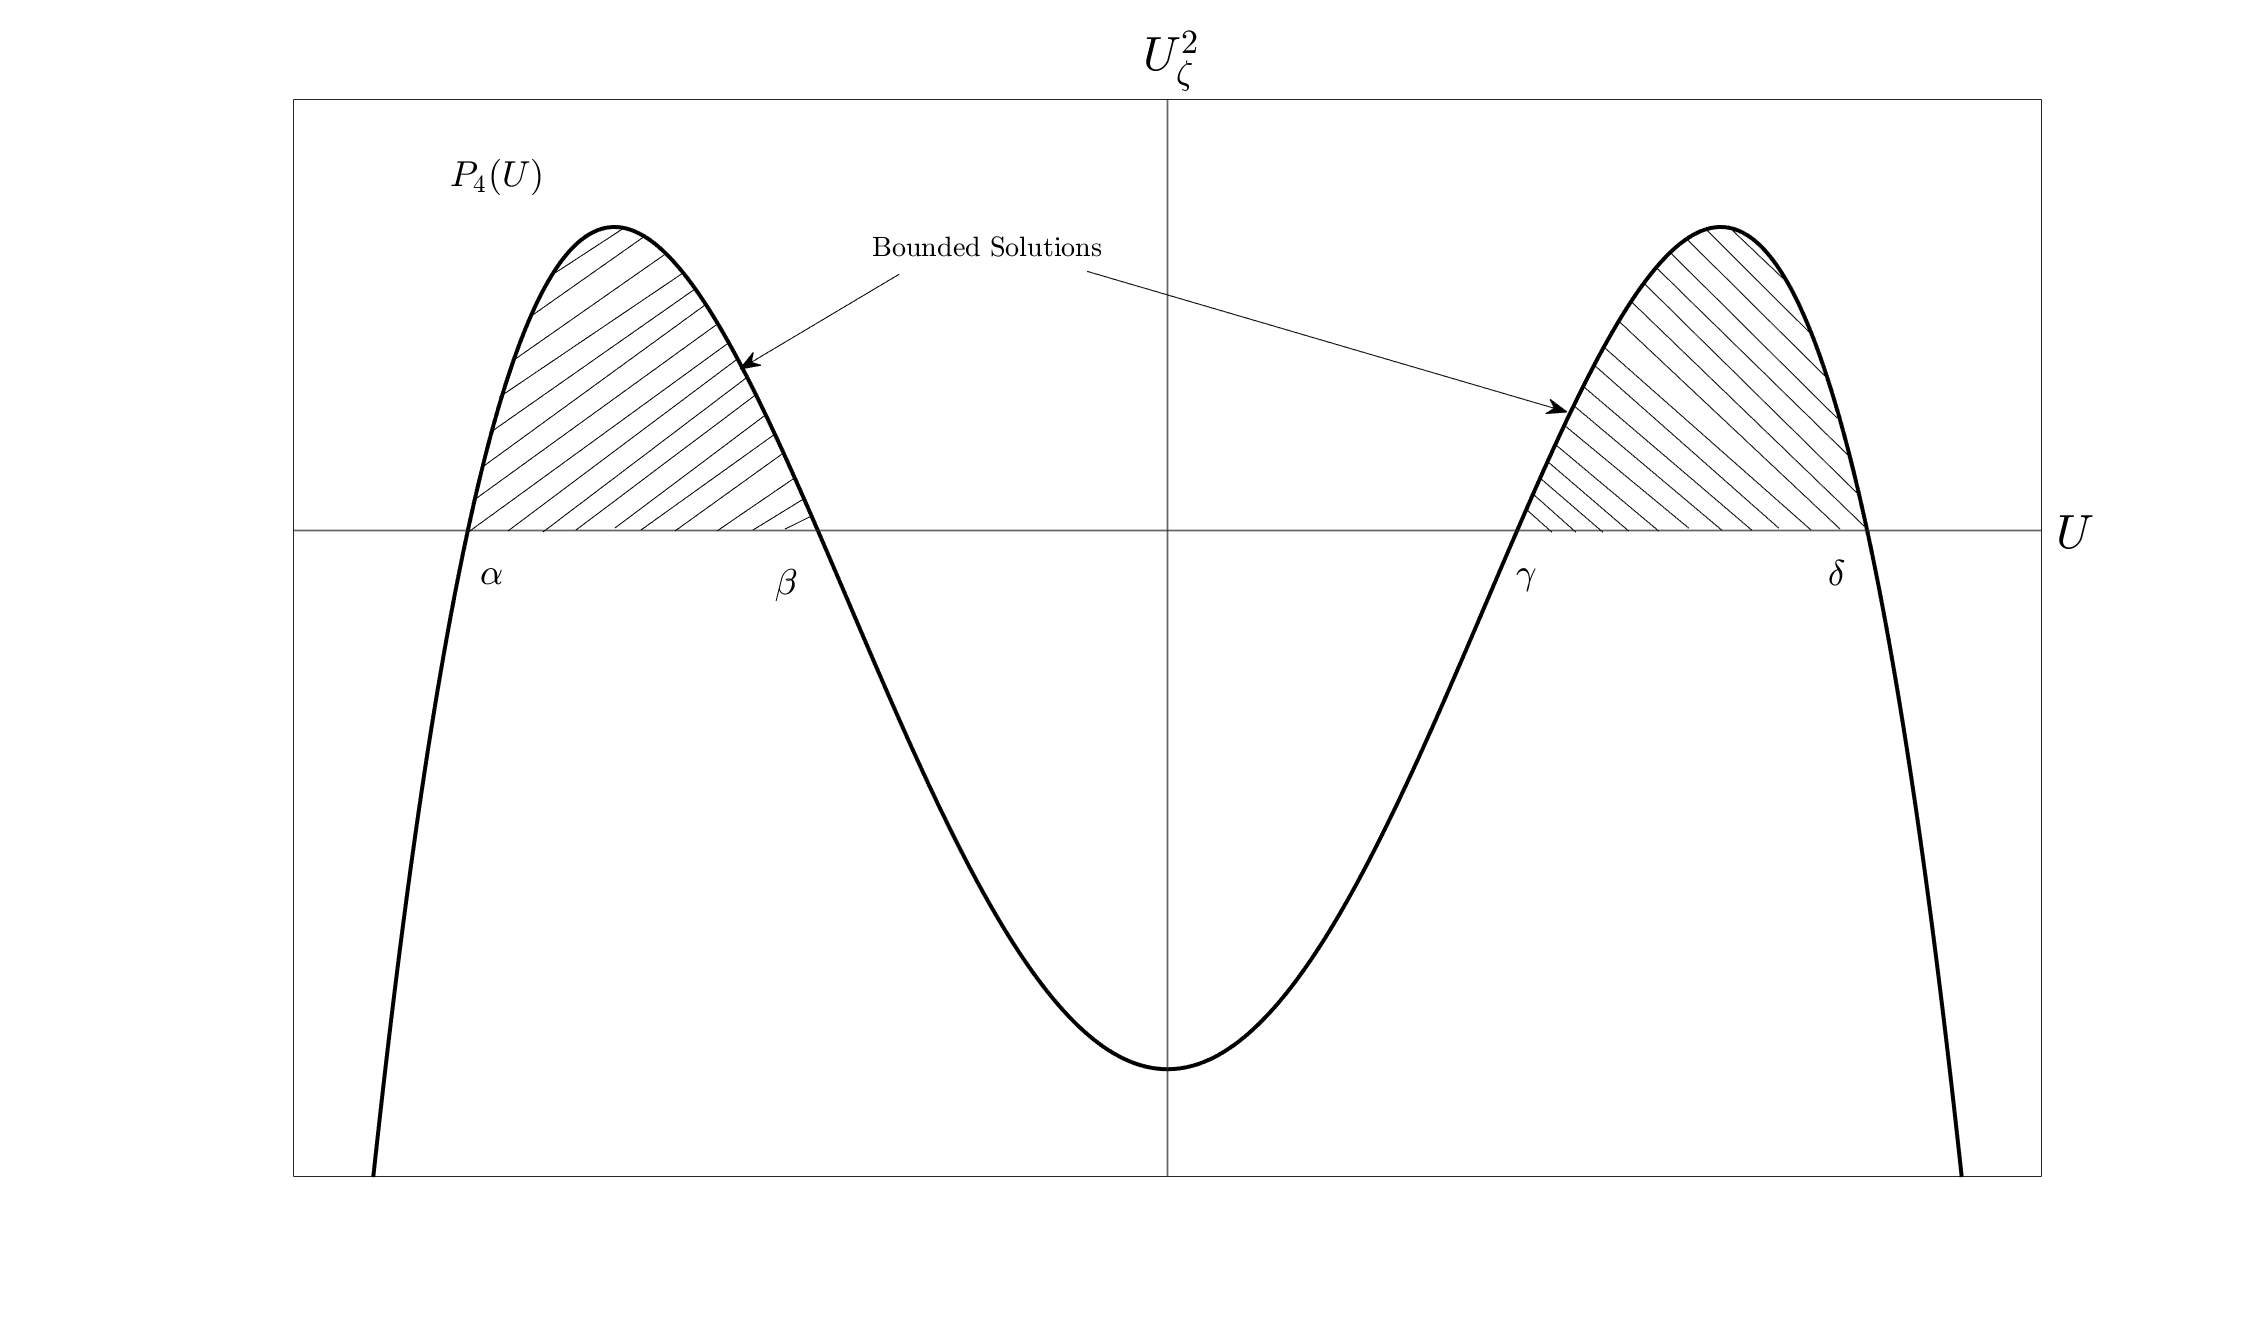
\includegraphics[scale = 0.2]{P4_nlw.png}
        \end{center}
        The above figure shows the general shape of $P_4(U)$. To find bounded solutions, we restrict $U \in (\alpha, \beta)$ or $U \in(\gamma, \delta)$. To this end, consider $U\in (\alpha,\beta)$. Then from our work above, we have
        \begin{align*}
            \left(\frac{\partial U}{\partial \zeta}\right)^2 &= -(U-\alpha)(U-\beta)(U-\gamma)(U-\delta)\\
            \implies \frac{\partial U}{\partial \zeta} &= \pm\sqrt{(U-\alpha)(U-\beta)(U-\gamma)(\delta-U)}
        \end{align*}
        We consider the positive case and note that this is a separable equation. Separating gives
        \begin{align*}
            \int_{\alpha}^{u}\frac{dU}{\sqrt{(U-\alpha)(U-\beta)(U-\gamma)(\delta - U)}} &= \int_{0}^{\zeta} d\zeta\\
            \implies \int_{\alpha}^{u}\frac{dU}{\sqrt{(U-\alpha)(U-\beta)(U-\gamma)(\delta - U)}} &= \zeta.
        \end{align*}
        Above we assumed $U(0) = \alpha$. This may be achieved by a simple shift of $\zeta$.
        For the integral on the left hand side, make the substitution $y = A\sqrt{\frac{U - \alpha}{\beta - U}}$ where $A$ is a constant to be determined. Solving for $U$ gives
        \begin{align*}
            \frac{y^2}{A^2} &= \frac{U - \alpha}{\beta - U}\\
            \implies (\beta - U)\frac{y^2}{A^2} &= U- \alpha\\
            \implies \alpha + \beta\frac{y^2}{A^2} &= \left(1 + \frac{y^2}{A^2}\right)U\\
            \implies U &= \frac{\alpha + \beta \frac{y^2}{A^2}}{1 + \frac{y^2}{A^2}}.
        \end{align*}
        Then
        \begin{align*}
            dU &= \frac{2\frac{\beta}{A^2}y\left(1 + \frac{y^2}{A^2}\right) - 2\frac{1}{A^2}y\left(\alpha + \beta\frac{y^2}{A^2}\right)}{\left(1 + \frac{y^2}{A^2}\right)^2}dy\\
            &= \frac{\frac{2\beta}{A^2}y + \frac{2\beta}{A^4}y^3 - \frac{2\alpha}{A^2}y - \frac{2\beta}{A^4}y^3}{\left(1 + \frac{y^2}{A^2}\right)^2}dy\\
            &= \frac{\frac{2}{A^2}(\beta - \alpha)y}{\left(1 + \frac{y^2}{A^2}\right)^2}dy.
        \end{align*}
        Thus the integral becomes
        \begin{align*}
            &\frac{2}{A^2}\int_0^{A\sqrt{\frac{u - \alpha}{\beta - u}}}\frac{(\beta - \alpha)y\left(1 + \frac{y^2}{A^2}\right)^{-2}}{\sqrt{\left(\frac{\alpha + \beta y^2/A^2}{1 + y^2/A^2} - \alpha\right)\left(\frac{\alpha + \beta y^2/A^2}{1 + y^2/A^2} - \beta\right)\left(\frac{\alpha + \beta y^2/A^2}{1 + y^2/A^2} - \gamma\right)\left(\delta - \frac{\alpha + \beta y^2/A^2}{1 + y^2/A^2}\right)}}dy = \\
            &= \frac{2}{A^2}\int_0^{A\sqrt{\frac{u - \alpha}{\beta - u}}}\frac{(\beta - \alpha)y}{\sqrt{\left(\alpha + \beta \frac{y^2}{A^2}- \alpha - \alpha \frac{y^2}{A^2}\right)\left(\alpha + \beta \frac{y^2}{A^2} - \beta - \beta \frac{y^2}{A^2}\right)\left(\alpha + \beta \frac{y^2}{A^2} - \gamma - \gamma \frac{y^2}{A^2}\right)\left(\delta + \delta \frac{y^2}{A^2} - \alpha - \beta \frac{y^2}{A^2}\right)}}dy\\
            &= \frac{2}{A^2}\int_0^{A\sqrt{\frac{u - \alpha}{\beta - u}}}\frac{(\beta - \alpha)y}{(\beta - \alpha)y/A\sqrt{\left([\gamma - \alpha] + [\gamma - \beta]y^2/A^2\right)\left([\delta - \alpha] + [\delta - \beta]y^2/A^2\right)}}dy\\
            &= \frac{2}{A\sqrt{(\gamma - \alpha)(\delta - \beta)}}\int_0^{A\sqrt{\frac{u - \alpha}{\beta - u}}}\frac{dy}{\sqrt{\left(1+ \frac{\gamma - \beta}{\gamma - \alpha}\frac{y^2}{A^2}\right)\left(1 + \frac{\delta - \beta}{\delta - \alpha}\frac{y^2}{A^2}\right)}}.
        \end{align*}
        From here, we take $A$ such that $\frac{\delta - \beta}{\delta - \alpha}\frac{1}{A^2} = 1 \implies A = \sqrt{\frac{\delta - \beta}{\delta - \alpha}}$. Then the above integral becomes
        \begin{align*}
            &\frac{2\sqrt{\delta - \alpha}}{\sqrt{\gamma - \alpha}\sqrt{\delta - \alpha}\sqrt{\delta - \beta}}\int_0^{\sqrt{\frac{(\delta - \beta)(u - \alpha)}{(\delta - \alpha)(\beta - u)}}} \frac{dy}{\sqrt{(1 + y^2)\left(1 + \frac{\gamma - \beta}{\gamma - \alpha}\frac{\delta - \alpha}{\delta - \beta}y^2\right)}} =\\
            &= \frac{2}{\sqrt{\gamma - \alpha}\sqrt{\delta - \beta}}\int_0^{\sqrt{\frac{(\delta - \beta)(u - \alpha)}{(\delta - \alpha)(\beta - u)}}}\frac{dy}{\sqrt{(1 + y^2)(1 + m'y^2)}}
        \end{align*}
        where $m' = \left(\frac{\gamma - \beta}{\gamma - \alpha}\right)\left(\frac{\delta - \alpha}{\delta - \beta}\right)$. Now let $y = \tan(\theta)$, $dt = \sec^2(\theta)d\theta$. Then the above integral becomes
        \begin{align*}
            &\frac{2}{\sqrt{\gamma - \alpha}\sqrt{\delta - \beta}}\int_0^{\arctan\left(\sqrt{\frac{(\delta - \beta)(u - \alpha)}{(\delta - \alpha)(\beta - u)}}\right)} \frac{\sec^2(\theta)d\theta}{\sqrt{(1 + \tan^2(\theta))(1 + m'\tan^2(\theta))}}\\
            &= \frac{2}{\sqrt{\gamma - \alpha}\sqrt{\delta - \beta}}\int_0^{\arctan\left(\sqrt{\frac{(\delta - \beta)(u - \alpha)}{(\delta - \alpha)(\beta - u)}}\right)}\frac{\sec(\theta)}{\sqrt{(1 + m'\tan^2(\theta))}}d\theta\\
            &= \frac{2}{\sqrt{\gamma - \alpha}\sqrt{\delta - \beta}}\int_0^{\arctan\left(\sqrt{\frac{(\delta - \beta)(u - \alpha)}{(\delta - \alpha)(\beta - u)}}\right)}\frac{\sec(\theta)}{\sqrt{(1  + \tan^2(\theta) - m\tan^2(\theta))}}d\theta\\
            &= \frac{2}{\sqrt{\gamma - \alpha}\sqrt{\delta - \beta}}\int_0^{\arctan\left(\sqrt{\frac{(\delta - \beta)(u - \alpha)}{(\delta - \alpha)(\beta - u)}}\right)}\frac{\sec(\theta)}{\sqrt{\sec^2(\theta) - m\tan^2(\theta)}}d\theta\\
            &= \frac{2}{\sqrt{\gamma - \alpha}\sqrt{\delta - \beta}}\int_0^{\arctan\left(\sqrt{\frac{(\delta - \beta)(u - \alpha)}{(\delta - \alpha)(\beta - u)}}\right)}\frac{d\theta}{\sqrt{1 - m\sin^2(\theta)}}\\
            &= \frac{2}{\sqrt{\gamma - \alpha}\sqrt{\delta - \beta}}F\left(\tan^{-1}\left(\sqrt{\frac{(\delta - \beta)(u - \alpha)}{(\delta - \alpha)(\beta - u)}}\right); m\right)
        \end{align*}
        
        where $F(y,m)$ is the first elliptic integral with modulus $m = 1 - m'$. Using this, the solution to the ODE is given as
        \begin{align*}
            \frac{2}{\sqrt{\gamma - \alpha}\sqrt{\delta - \beta}}F\left(\tan^{-1}\left(\sqrt{\frac{(\delta - \beta)(u - \alpha)}{(\delta - \alpha)(\beta - u)}}\right);m\right) &= \zeta\\
            F\left(\tan^{-1}\left(\sqrt{\frac{(\delta - \beta)(u - \alpha)}{(\delta - \alpha)(\beta - u)}}\right);m\right) &= \frac{\sqrt{\gamma - \alpha}\sqrt{\delta - \beta}}{2}\zeta\\
            \implies \tan^{-1}\left(\sqrt{\frac{(\delta - \beta)(u - \alpha)}{(\delta - \alpha)(\beta - u)}}\right) &= \text{am}\left(\frac{\sqrt{\gamma - \alpha}\sqrt{\delta - \beta}}{2}\zeta;m\right)\\
            \implies \sqrt{\frac{(\delta - \beta)(u - \alpha)}{(\delta - \alpha)(\beta - u)}} &= \frac{\text{sn}\left(\frac{\sqrt{\gamma - \alpha}\sqrt{\delta - \beta}}{2}\zeta; m\right)}{\text{cn}\left(\frac{\sqrt{\gamma - \alpha}\sqrt{\delta - \beta}}{2}\zeta; m\right)}\\
            \implies \frac{(\delta - \alpha)(u - \alpha)}{(\delta - \alpha)(\beta - u)} &= \frac{\text{sn}^2\left(\frac{\sqrt{\gamma - \alpha}\sqrt{\delta - \beta}}{2}\zeta; m\right)}{\text{cn}^2\left(\frac{\sqrt{\gamma - \alpha}\sqrt{\delta - \beta}}{2}\zeta; m\right)}\\
            \implies \frac{u - \alpha}{\beta - u} &= \frac{\delta - \alpha}{\delta - \beta}\frac{\text{sn}^2\left(\frac{\sqrt{\gamma - \alpha}\sqrt{\delta - \beta}}{2}\zeta; m\right)}{\text{cn}^2\left(\frac{\sqrt{\gamma - \alpha}\sqrt{\delta - \beta}}{2}\zeta; m\right)}\\
            \implies u - \alpha &= (\beta - u)\frac{\delta - \alpha}{\delta - \beta}\frac{\text{sn}^2\left(\frac{\sqrt{\gamma - \alpha}\sqrt{\delta - \beta}}{2}\zeta; m\right)}{\text{cn}^2\left(\frac{\sqrt{\gamma - \alpha}\sqrt{\delta - \alpha}}{2}\zeta; m\right)}\\
            \implies u\left(1 + \frac{\delta - \alpha}{\delta - \beta}\right)\frac{\text{sn}^2\left(\frac{\sqrt{\gamma - \alpha}\sqrt{\delta - \beta}}{2}\zeta; m\right)}{\text{cn}^2\left(\frac{\sqrt{\gamma - \alpha}\sqrt{\delta - \beta}}{2}\zeta; m\right)} &= \alpha + \beta\frac{\delta - \alpha}{\delta - \beta}\frac{\text{sn}^2\left(\frac{\sqrt{\gamma - \alpha}\sqrt{\delta - \beta}}{2}\zeta; m\right)}{\text{cn}^2\left(\frac{\sqrt{\gamma - \alpha}\sqrt{\delta - \beta}}{2}\zeta; m\right)}
        \end{align*}
        \[\implies u = \frac{\alpha\text{cn}^2\left(\frac{\sqrt{\gamma - \alpha}\sqrt{\delta - \beta}}{2}\zeta; m\right) + \beta\frac{\delta - \alpha}{\delta - \beta}\text{sn}^2\left(\frac{\sqrt{\gamma - \alpha}\sqrt{\delta - \beta}}{2}\zeta;m\right)}{\text{cn}^2\left(\frac{\sqrt{\gamma - \alpha}\sqrt{\delta - \beta}}{2}\zeta; m\right) + \frac{\delta - \alpha}{\delta - \beta}\text{sn}^2\left(\frac{\sqrt{\gamma - \alpha}\sqrt{\delta - \beta}}{2}\zeta;m\right)}\]
        where $\text{am}(\cdot;\cdot)$ is the elliptic amplitude function, $\text{sn}(\cdot;\cdot)$ is the elliptic sine function, and $\text{cn}(\cdot;\cdot)$ is the elliptic cosine function

        \item[(b)] Find all bounded solitary wave solutions.
        \newline\newline
        \textit{Soln.} In the limiting case $\gamma \to \beta$, notice $m \to 1$. And as $m \to 1$, $\text{cn}(y;m) \to \text{sech}(y)$ and $\text{sn}(y;m) \to \tanh(y)$, so that as $m \to 1$,
        \[u \to \frac{\alpha\text{sech}^2\left(\frac{\sqrt{\beta - \alpha}\sqrt{\delta - \beta}}{2}\zeta\right) + \beta\frac{\delta - \alpha}{\delta - \beta}\tanh^2\left(\frac{\sqrt{\beta - \alpha}\sqrt{\delta - \beta}}{2}\zeta\right)}{\text{sech}^2\left(\frac{\sqrt{\beta - \alpha}\sqrt{\delta - \beta}}{2}\zeta\right) + \frac{\delta - \alpha}{\delta - \beta}\tanh^2\left(\frac{\sqrt{\beta - \alpha}\sqrt{\delta - \beta}}{2}\zeta\right)}\]

        \begin{figure}[H]
            \centering
            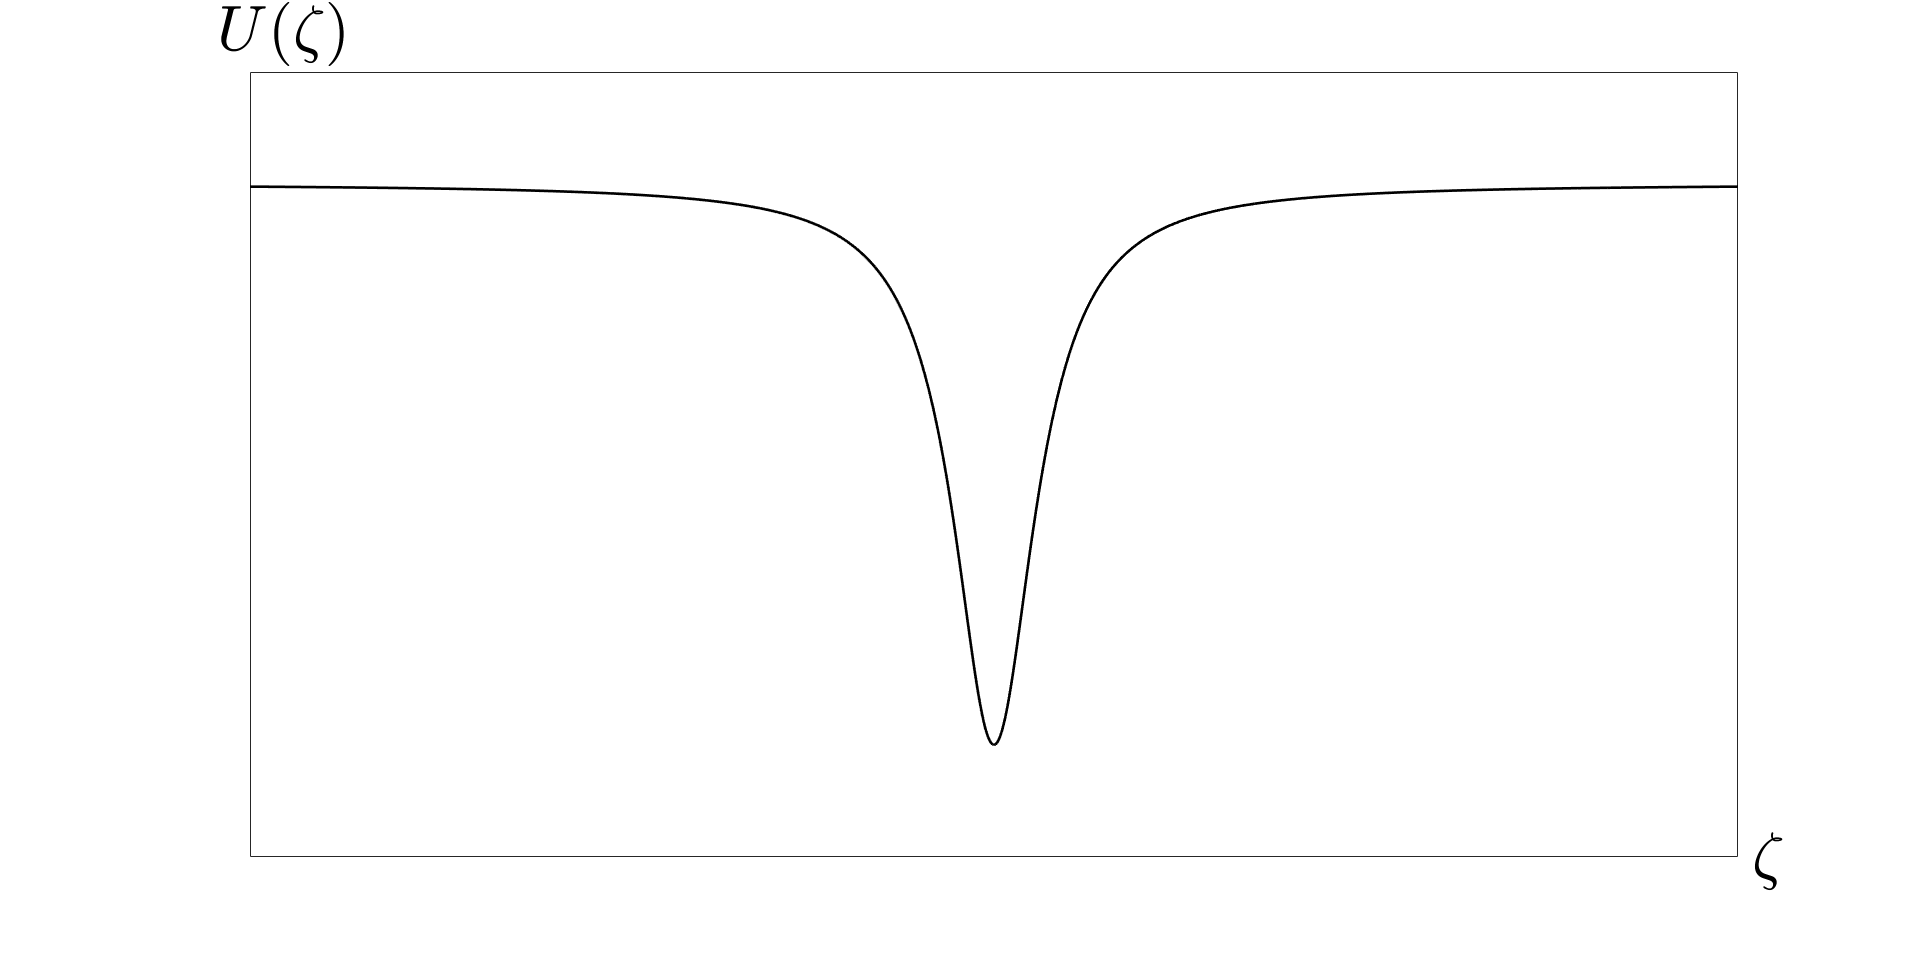
\includegraphics[scale = 0.3]{soliton1_mkdv.png}
            \caption{Example displaying the shape of the above solution.}
        \end{figure}
    \end{itemize}
\end{itemize}

\end{document}
